\documentclass[10pt,a4paper]{article}
\usepackage[utf8]{inputenc}
\usepackage[top=2cm,bottom=2cm,left=2cm,right=2cm]{geometry}
\usepackage{amsmath}
\usepackage{amssymb}
\usepackage{array}
\usepackage{tikz}
\usetikzlibrary{arrows.meta,calc,patterns,positioning}
\usepackage{pgfplots}
\pgfplotsset{compat=1.18}
\usepackage[dvipsnames,svgnames]{xcolor}
\usepackage{hyperref}

% Anchor persamaan unik meski nomor di-reset per blok.
\newcounter{eqblock}
\newcommand{\reseteq}{%
  \stepcounter{eqblock}%
  \setcounter{equation}{0}%
  \renewcommand{\theHequation}{\arabic{eqblock}.\arabic{equation}}%
}

\pgfplotsset{
  grafik/.style={
    axis lines=middle,
    xlabel={$x$}, ylabel={$y$},
    width=7.5cm, height=6cm,
    grid=major, grid style={gray!25},
    tick label style={font=\scriptsize},
    every axis x label/.style={at={(ticklabel* cs:1)},anchor=west},
    every axis y label/.style={at={(ticklabel* cs:1)},anchor=south},
    title style={yshift=2ex},
  },
}

\title{Tugas Minggu 3 : Fungsi}
\author{Matematika untuk Sistem Informasi}
\date{}

\begin{document}

\maketitle

\begin{enumerate}

%===========================================================
\item Tentukan daerah asal (domain) dan daerah hasil (range) dari fungsi berikut:
\begin{enumerate}

%-----------------------------------------------------------
\item $f(x) = \sqrt{9 - x}$

\textbf{Jawab:}
\begin{itemize}
\item \textbf{Langkah 1: Identifikasi Jenis Fungsi}

$f(x) = \sqrt{9 - x}$ memuat akar kuadrat, sehingga radikan (bilangan di bawah akar) harus non-negatif.
% concept: radikan non-negatif karena akar kuadrat

\item \textbf{Langkah 2: Tentukan Domain}

\reseteq
\begin{align}
9 - x &\geq 0 \quad \text{(Syarat akar kuadrat)} \\
-x &\geq -9 \quad \text{(Kurangi 9 pada kedua ruas)} \\
x &\leq 9 \quad \text{(Kali kedua ruas dengan $-1$, tanda berubah)} \\
D_f &= \{x \in \mathbb{R} \mid x \leq 9\} = (-\infty, 9] \quad \text{(Kesimpulan domain)}
\end{align}

\item \textbf{Langkah 3: Tentukan Range}

\reseteq
\begin{align}
\sqrt{9 - x} &\geq 0 \quad \text{(Sifat akar untuk $x \leq 9$)} \\
f(9) &= \sqrt{9 - 9} = 0 \quad \text{(Nilai minimum tercapai di $x = 9$)}
\end{align}
Ketika $x$ semakin kecil, $9 - x$ membesar tanpa batas sehingga $f(x)$ juga membesar tanpa batas. Jadi
\[
R_f = \{y \in \mathbb{R} \mid y \geq 0\} = [0, \infty).
\]

\item \textbf{Langkah 4: Verifikasi dengan Grafik}

\begin{center}
\begin{tabular}{c|ccccc}
$x$ & $-7$ & $0$ & $5$ & $8$ & $9$ \\ \hline
$f(x)$ & $4$ & $3$ & $2$ & $1$ & $0$
\end{tabular}
\end{center}

\begin{center}
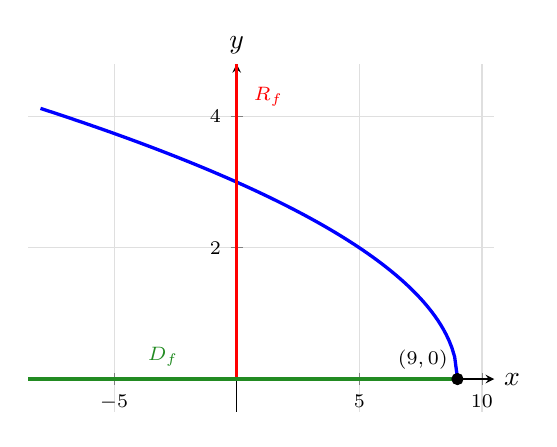
\begin{tikzpicture}
\begin{axis}[grafik, xmin=-8.5, xmax=10.5, ymin=-0.5, ymax=4.8]
  \addplot[very thick, blue, domain=-8:9, samples=150] {sqrt(9-x)};
  \draw[very thick, Red] (axis cs:0,0) -- (axis cs:0,4.8);
  \draw[very thick, ForestGreen] (axis cs:-8.5,0) -- (axis cs:9,0);
  \filldraw[black] (axis cs:9,0) circle (2pt) node[above left,font=\scriptsize] {$(9,0)$};
  \node[Red,font=\scriptsize,anchor=west] at (axis cs:0.3,4.3) {$R_f$};
  \node[ForestGreen,font=\scriptsize,anchor=south] at (axis cs:-3,0.05) {$D_f$};
\end{axis}
\end{tikzpicture}
\end{center}
Garis hijau pada sumbu-$x$ menunjukkan domain $(-\infty, 9]$ dan garis merah pada sumbu-$y$ menunjukkan range $[0, \infty)$.
% value_table: (-7, 4); (0, 3); (5, 2); (8, 1); (9, 0)
% final: D_f = (-\infty, 9]
% final: R_f = [0, \infty)
\end{itemize}

%-----------------------------------------------------------
\item $f(x) = x^2 - 3x - 4$

\textbf{Jawab:}
\begin{itemize}
\item \textbf{Langkah 1: Identifikasi Jenis Fungsi}

$f(x) = x^2 - 3x - 4$ adalah fungsi kuadrat (polinom derajat 2) dengan $a = 1$, $b = -3$, $c = -4$. Karena $a > 0$, parabola terbuka ke atas.
% concept: fungsi kuadrat; parabola terbuka ke atas ($a > 0$)

\item \textbf{Langkah 2: Tentukan Domain}

\reseteq
\begin{align}
&\text{Polinom terdefinisi untuk semua bilangan real} \quad \text{(Tidak ada syarat)} \\
&D_f = \{x \in \mathbb{R}\} = (-\infty, \infty) \quad \text{(Kesimpulan domain)}
\end{align}

\item \textbf{Langkah 3: Tentukan Range}

Titik puncak parabola:
\reseteq
\begin{align}
x_p &= \frac{-b}{2a} = \frac{-(-3)}{2(1)} = \frac{3}{2} \quad \text{(Absis titik puncak)} \\
f\left(\frac{3}{2}\right) &= \left(\frac{3}{2}\right)^2 - 3\left(\frac{3}{2}\right) - 4 \quad \text{(Substitusi $x = \tfrac{3}{2}$)} \\
&= \frac{9}{4} - \frac{18}{4} - \frac{16}{4} = -\frac{25}{4} \quad \text{(Nilai minimum)}
\end{align}
Dengan melengkapkan kuadrat, $f(x) = \left(x - \frac{3}{2}\right)^2 - \frac{25}{4} \geq -\frac{25}{4}$ karena $\left(x - \frac{3}{2}\right)^2 \geq 0$.
Untuk $x \to \pm\infty$ nilai $f(x)$ membesar tanpa batas, sehingga
\[
R_f = \left\{y \in \mathbb{R} \;\middle|\; y \geq -\frac{25}{4}\right\} = \left[-\frac{25}{4}, \infty\right).
\]

\item \textbf{Langkah 4: Verifikasi dengan Grafik}

Bentuk faktor $f(x) = (x - 4)(x + 1)$ memberi titik potong sumbu-$x$ di $(-1, 0)$ dan $(4, 0)$.
\begin{center}
\begin{tabular}{c|ccccc}
$x$ & $-1$ & $0$ & $\frac{3}{2}$ & $3$ & $4$ \\ \hline
$f(x)$ & $0$ & $-4$ & $-\frac{25}{4}$ & $-4$ & $0$
\end{tabular}
\end{center}

\begin{center}
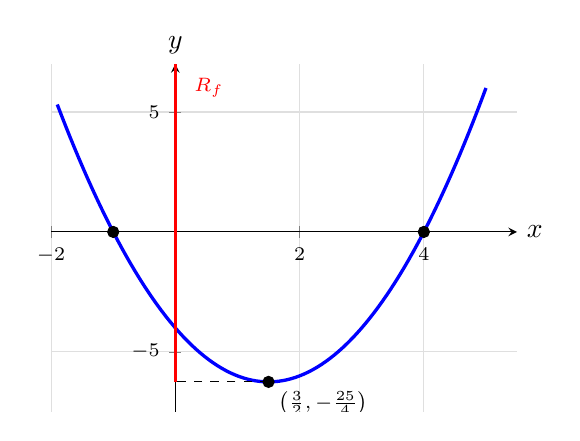
\begin{tikzpicture}
\begin{axis}[grafik, xmin=-2, xmax=5.5, ymin=-7.5, ymax=7]
  \addplot[very thick, blue, domain=-1.9:5, samples=100] {x^2-3*x-4};
  \draw[very thick, Red] (axis cs:0,-6.25) -- (axis cs:0,7);
  \draw[dashed] (axis cs:1.5,-6.25) -- (axis cs:0,-6.25);
  \filldraw[black] (axis cs:1.5,-6.25) circle (2pt) node[below right,font=\scriptsize] {$\left(\frac{3}{2},-\frac{25}{4}\right)$};
  \filldraw[black] (axis cs:-1,0) circle (2pt);
  \filldraw[black] (axis cs:4,0) circle (2pt);
  \node[Red,font=\scriptsize,anchor=west] at (axis cs:0.15,6) {$R_f$};
\end{axis}
\end{tikzpicture}
\end{center}
Titik terendah grafik adalah $\left(\frac{3}{2}, -\frac{25}{4}\right)$, dan garis merah pada sumbu-$y$ menunjukkan range $\left[-\frac{25}{4}, \infty\right)$.
% value_table: (-1, 0); (0, -4); (3/2, -25/4); (3, -4); (4, 0)
% final: D_f = (-\infty, \infty)
% final: R_f = \left[-\frac{25}{4}, \infty\right)
\end{itemize}

\end{enumerate}

%===========================================================
\item Gambarkan grafik
\[
f(x) =
\begin{cases}
  x + 1, & x < -1 \\
  x^2, & -1 \le x < 2 \\
  2 - x, & x \ge 2
\end{cases}
\]

\textbf{Jawab:}
\begin{itemize}
\item \textbf{Langkah 1: Identifikasi Setiap Potongan}

\begin{center}
\begin{tabular}{c|c|c}
untuk $x < -1$ & untuk $-1 \le x < 2$ & untuk $x \ge 2$ \\ \hline
$f(x) = x + 1$ & $f(x) = x^2$ & $f(x) = 2 - x$ \\
garis lurus (naik) & parabola & garis lurus (turun)
\end{tabular}
\end{center}

\item \textbf{Langkah 2: Periksa Titik Ujung Selang}

\reseteq
\begin{align}
x \to -1^{-}: \quad &f(x) = x + 1 \to 0 \quad \text{(Potongan pertama, titik kosong $(-1,0)$)} \\
x = -1: \quad &f(-1) = (-1)^2 = 1 \quad \text{(Potongan kedua, titik penuh $(-1,1)$)} \\
x \to 2^{-}: \quad &f(x) = x^2 \to 4 \quad \text{(Potongan kedua, titik kosong $(2,4)$)} \\
x = 2: \quad &f(2) = 2 - 2 = 0 \quad \text{(Potongan ketiga, titik penuh $(2,0)$)}
\end{align}
Grafik \emph{melompat} di $x = -1$ (dari ketinggian $0$ ke $1$) dan di $x = 2$ (dari ketinggian $4$ ke $0$).
% concept: grafik melompat di titik ujung selang (titik kosong vs penuh)

\item \textbf{Langkah 3: Tabel Nilai}

\begin{center}
\begin{tabular}{c|c|c}
$x$ & Potongan & $f(x)$ \\ \hline
$-3$ & $x + 1$ & $-2$ \\
$-2$ & $x + 1$ & $-1$ \\
$-1$ & $x^2$ & $1$ \\
$0$ & $x^2$ & $0$ \\
$1$ & $x^2$ & $1$ \\
$1{,}5$ & $x^2$ & $2{,}25$ \\
$2$ & $2 - x$ & $0$ \\
$3$ & $2 - x$ & $-1$ \\
$4$ & $2 - x$ & $-2$
\end{tabular}
\end{center}

\item \textbf{Langkah 4: Gambar Grafik}

\begin{center}
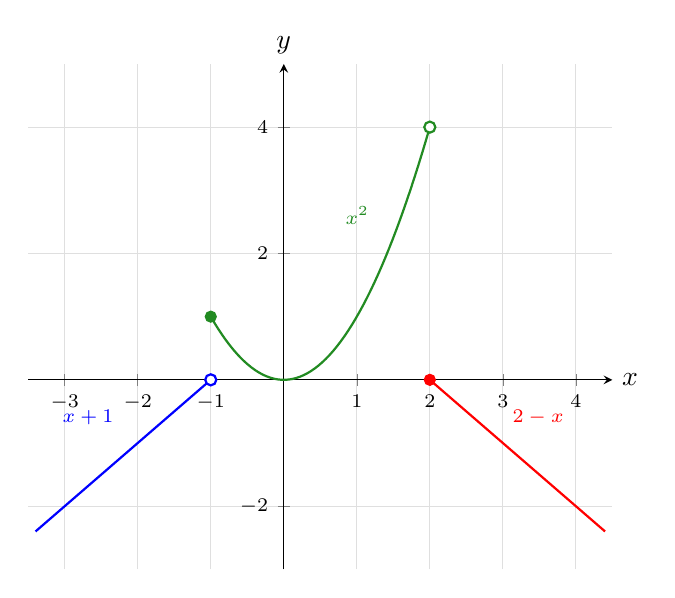
\begin{tikzpicture}
\begin{axis}[grafik, width=9cm, height=8cm, xmin=-3.5, xmax=4.5, ymin=-3, ymax=5]
  \addplot[domain=-3.4:-1, thick, blue] {x+1};
  \addplot[domain=-1:2, samples=60, thick, ForestGreen] {x^2};
  \addplot[domain=2:4.4, thick, Red] {2-x};
  \filldraw[blue, fill=white, thick] (axis cs:-1,0) circle (2pt);
  \filldraw[ForestGreen] (axis cs:-1,1) circle (2pt);
  \filldraw[ForestGreen, fill=white, thick] (axis cs:2,4) circle (2pt);
  \filldraw[Red] (axis cs:2,0) circle (2pt);
  \node[font=\scriptsize, blue, anchor=east] at (axis cs:-2.2,-0.6) {$x + 1$};
  \node[font=\scriptsize, ForestGreen, anchor=east] at (axis cs:1.3,2.6) {$x^2$};
  \node[font=\scriptsize, Red, anchor=west] at (axis cs:3,-0.6) {$2 - x$};
\end{axis}
\end{tikzpicture}
\end{center}

\item \textbf{Langkah 5: Domain dan Range}

\reseteq
\begin{align}
D_f &= (-\infty, -1) \cup [-1, 2) \cup [2, \infty) = \mathbb{R} \quad \text{(Gabungan selang)} \\
x < -1 &\;\Rightarrow\; x + 1 < 0 \quad \text{(Potongan pertama memberi $(-\infty, 0)$)} \\
-1 \le x < 2 &\;\Rightarrow\; 0 \le x^2 < 4 \quad \text{(Potongan kedua memberi $[0, 4)$, minimum di $x = 0$)} \\
x \ge 2 &\;\Rightarrow\; 2 - x \le 0 \quad \text{(Potongan ketiga memberi $(-\infty, 0]$)}
\end{align}
Sehingga
\[
R_f = (-\infty, 0) \cup [0, 4) \cup (-\infty, 0] = (-\infty, 4).
\]
% final: D_f = \mathbb{R}
% final: R_f = (-\infty, 4)
% graph_points: (-1, 0, open); (-1, 1, closed); (2, 4, open); (2, 0, closed)
\end{itemize}

%===========================================================
\item Gambarkan grafik
\[
f(x) =
\begin{cases}
  x, & x \le -1 \\
  x^2, & -1 < x < 2 \\
  3, & x \ge 2
\end{cases}
\]

\textbf{Jawab:}
\begin{itemize}
\item \textbf{Langkah 1: Identifikasi Setiap Potongan}

\begin{center}
\begin{tabular}{c|c|c}
untuk $x \le -1$ & untuk $-1 < x < 2$ & untuk $x \ge 2$ \\ \hline
$f(x) = x$ & $f(x) = x^2$ & $f(x) = 3$ \\
garis lurus (naik) & parabola & garis mendatar
\end{tabular}
\end{center}

\item \textbf{Langkah 2: Periksa Titik Ujung Selang}

\reseteq
\begin{align}
x = -1: \quad &f(-1) = -1 \quad \text{(Potongan pertama, titik penuh $(-1,-1)$)} \\
x \to -1^{+}: \quad &f(x) = x^2 \to 1 \quad \text{(Potongan kedua, titik kosong $(-1,1)$)} \\
x \to 2^{-}: \quad &f(x) = x^2 \to 4 \quad \text{(Potongan kedua, titik kosong $(2,4)$)} \\
x = 2: \quad &f(2) = 3 \quad \text{(Potongan ketiga, titik penuh $(2,3)$)}
\end{align}
Grafik \emph{melompat} di $x = -1$ (dari ketinggian $-1$ ke $1$) dan di $x = 2$ (dari ketinggian $4$ ke $3$).
% concept: grafik melompat di titik ujung selang (titik kosong vs penuh)

\item \textbf{Langkah 3: Tabel Nilai}

\begin{center}
\begin{tabular}{c|c|c}
$x$ & Potongan & $f(x)$ \\ \hline
$-3$ & $x$ & $-3$ \\
$-2$ & $x$ & $-2$ \\
$-1$ & $x$ & $-1$ \\
$0$ & $x^2$ & $0$ \\
$1$ & $x^2$ & $1$ \\
$1{,}5$ & $x^2$ & $2{,}25$ \\
$2$ & $3$ & $3$ \\
$3$ & $3$ & $3$
\end{tabular}
\end{center}

\item \textbf{Langkah 4: Gambar Grafik}

\begin{center}
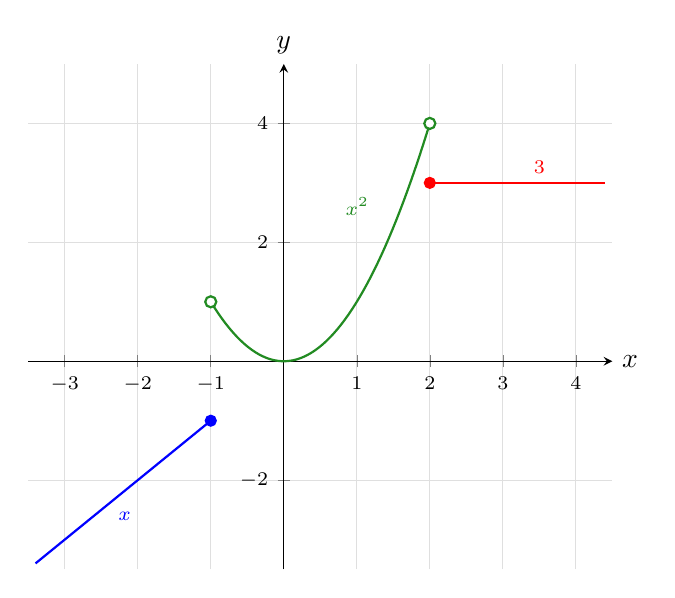
\begin{tikzpicture}
\begin{axis}[grafik, width=9cm, height=8cm, xmin=-3.5, xmax=4.5, ymin=-3.5, ymax=5]
  \addplot[domain=-3.4:-1, thick, blue] {x};
  \addplot[domain=-1:2, samples=60, thick, ForestGreen] {x^2};
  \addplot[domain=2:4.4, thick, Red] {3};
  \filldraw[blue] (axis cs:-1,-1) circle (2pt);
  \filldraw[ForestGreen, fill=white, thick] (axis cs:-1,1) circle (2pt);
  \filldraw[ForestGreen, fill=white, thick] (axis cs:2,4) circle (2pt);
  \filldraw[Red] (axis cs:2,3) circle (2pt);
  \node[font=\scriptsize, blue, anchor=west] at (axis cs:-2.4,-2.6) {$x$};
  \node[font=\scriptsize, ForestGreen, anchor=east] at (axis cs:1.3,2.6) {$x^2$};
  \node[font=\scriptsize, Red, anchor=south] at (axis cs:3.5,3) {$3$};
\end{axis}
\end{tikzpicture}
\end{center}

\item \textbf{Langkah 5: Domain dan Range}

\reseteq
\begin{align}
D_f &= (-\infty, -1] \cup (-1, 2) \cup [2, \infty) = \mathbb{R} \quad \text{(Gabungan selang)} \\
x \le -1 &\;\Rightarrow\; f(x) = x \le -1 \quad \text{(Potongan pertama memberi $(-\infty, -1]$)} \\
-1 < x < 2 &\;\Rightarrow\; 0 \le x^2 < 4 \quad \text{(Potongan kedua memberi $[0, 4)$, minimum di $x = 0$)} \\
x \ge 2 &\;\Rightarrow\; f(x) = 3 \quad \text{(Potongan ketiga memberi $\{3\}$)}
\end{align}
Karena $3 \in [0, 4)$, diperoleh
\[
R_f = (-\infty, -1] \cup [0, 4) \cup \{3\} = (-\infty, -1] \cup [0, 4).
\]
% final: D_f = \mathbb{R}
% final: R_f = (-\infty, -1] \cup [0, 4)
% graph_points: (-1, -1, closed); (-1, 1, open); (2, 4, open); (2, 3, closed)
\end{itemize}

%===========================================================
\item Diketahui $f(x) = \sqrt{x}$ dan $g(x) = x^2$.
\begin{enumerate}
\item Periksa apakah $(f \circ g)$ ada?

\textbf{Jawab:}
\begin{itemize}
\item \textbf{Langkah 1: Domain dan Range $f$ dan $g$}

\reseteq
\begin{align}
x \geq 0 &\;\Rightarrow\; D_f = [0, \infty) \quad \text{(Syarat akar)} \\
\sqrt{x} \geq 0,\ f(0) = 0 &\;\Rightarrow\; R_f = [0, \infty) \quad \text{(Akar non-negatif, naik tanpa batas)} \\
D_g &= \mathbb{R} \quad \text{(Polinom)} \\
x^2 \geq 0 &\;\Rightarrow\; R_g = [0, \infty) \quad \text{(Minimum $g(0) = 0$)}
\end{align}

\item \textbf{Langkah 2: Bagian (a), Periksa Syarat $f \circ g$}

\reseteq
\begin{align}
R_g \cap D_f &= [0, \infty) \cap [0, \infty) = [0, \infty) \neq \emptyset
\end{align}
Karena $R_g \cap D_f \neq \emptyset$, maka $f \circ g$ ada.
% concept: $f \circ g$ ada karena $R_g \cap D_f \neq \emptyset$
% final: \text{ada}
\end{itemize}

\item Jika ada, tentukan $(f \circ g)(x)$, $(f \circ g)(5)$, $D_{f \circ g}$, dan $R_{f \circ g}$.

\textbf{Jawab:}
\begin{itemize}
\item \textbf{Langkah 1: Domain dan Range $f$ dan $g$ (ringkas)}

\reseteq
\begin{align}
D_f &= [0, \infty),\quad R_f = [0, \infty) \\
D_g &= \mathbb{R},\quad R_g = [0, \infty)
\end{align}

\item \textbf{Langkah 2: Bagian (b), Rumus dan Nilai $f \circ g$}

\reseteq
\begin{align}
(f \circ g)(x) &= f\bigl(g(x)\bigr) = f(x^2) \quad \text{(Definisi komposisi)} \\
&= \sqrt{x^2} = |x| \quad \text{(Ganti $x$ pada $f$ dengan $x^2$; ingat $\sqrt{x^2} = |x|$)} \\
(f \circ g)(5) &= |5| = 5 \quad \text{(Substitusi $x = 5$)}
\end{align}
Perhatikan bahwa $\sqrt{x^2} = |x|$, bukan $x$. Misalnya untuk $x = -5$ diperoleh $\sqrt{(-5)^2} = \sqrt{25} = 5 = |-5|$, bukan $-5$.

\item \textbf{Langkah 3: Domain $f \circ g$}

\reseteq
\begin{align}
D_{f \circ g} &= \{x \in D_g \mid g(x) \in D_f\} \quad \text{(Definisi domain komposisi)} \\
&= \{x \in \mathbb{R} \mid x^2 \in [0, \infty)\} \\
x^2 &\geq 0 \quad \text{(Selalu benar untuk setiap $x \in \mathbb{R}$)}
\end{align}
Jadi $D_{f \circ g} = \mathbb{R} = (-\infty, \infty)$.

\item \textbf{Langkah 4: Range $f \circ g$}

\reseteq
\begin{align}
R_{f \circ g} &= \{ y \in R_f \mid y = f(t), \, t \in R_g \cap D_f \} \quad \text{(Rumus range komposisi)} \\
t &\in R_g \cap D_f = [0, \infty) \quad \text{(Masukan yang diterima $f$)} \\
y = f(t) = \sqrt{t},\ t \in [0, \infty) &\;\Rightarrow\; y \in [0, \infty) \quad \text{(Peta oleh $f$)}
\end{align}
\[
(f \circ g)(x) = |x|, \quad (f \circ g)(5) = 5, \quad D_{f \circ g} = (-\infty, \infty), \quad R_{f \circ g} = [0, \infty).
\]
% final: (f \circ g)(x) = |x|
% final: (f \circ g)(5) = 5
% final: D_{f \circ g} = (-\infty, \infty)
% final: R_{f \circ g} = [0, \infty)
\end{itemize}
\end{enumerate}

%===========================================================
\item Diketahui $f(x) = x^2$ dan $g(x) = x - 1$.
\begin{enumerate}
\item Periksa apakah $(g \circ f)$ ada?

\textbf{Jawab:}
\begin{itemize}
\item \textbf{Langkah 1: Domain dan Range $f$ dan $g$}

\reseteq
\begin{align}
D_f &= \mathbb{R} \quad \text{(Polinom)} \\
x^2 \geq 0 &\;\Rightarrow\; R_f = [0, \infty) \quad \text{(Minimum $f(0) = 0$)} \\
D_g &= \mathbb{R} \quad \text{(Polinom)} \\
R_g &= \mathbb{R} \quad \text{(Fungsi linear dengan gradien $1 \neq 0$)}
\end{align}

\item \textbf{Langkah 2: Bagian (a), Periksa Syarat $g \circ f$}

\reseteq
\begin{align}
R_f \cap D_g &= [0, \infty) \cap (-\infty, \infty) = [0, \infty) \neq \emptyset
\end{align}
Karena $R_f \cap D_g \neq \emptyset$, maka $g \circ f$ ada.
% concept: $g \circ f$ ada karena $R_f \cap D_g \neq \emptyset$
% final: \text{ada}
\end{itemize}

\item Jika ada, tentukan $(g \circ f)(x)$, $(g \circ f)(2)$, $D_{g \circ f}$, dan $R_{g \circ f}$.

\textbf{Jawab:}
\begin{itemize}
\item \textbf{Langkah 1: Domain dan Range $f$ dan $g$ (ringkas)}

\reseteq
\begin{align}
D_f &= \mathbb{R},\quad R_f = [0, \infty) \\
D_g &= \mathbb{R},\quad R_g = \mathbb{R}
\end{align}

\item \textbf{Langkah 2: Bagian (b), Rumus dan Nilai $g \circ f$}

\reseteq
\begin{align}
(g \circ f)(x) &= g\bigl(f(x)\bigr) = g(x^2) \quad \text{(Definisi komposisi)} \\
&= x^2 - 1 \quad \text{(Ganti $x$ pada $g$ dengan $x^2$)} \\
(g \circ f)(2) &= 2^2 - 1 = 3 \quad \text{(Substitusi $x = 2$)}
\end{align}

\item \textbf{Langkah 3: Domain $g \circ f$}

\reseteq
\begin{align}
D_{g \circ f} &= \{x \in D_f \mid f(x) \in D_g\} \quad \text{(Definisi domain komposisi)} \\
&= \{x \in \mathbb{R} \mid x^2 \in (-\infty, \infty)\} \\
x^2 &\in \mathbb{R} \quad \text{(Selalu benar untuk setiap $x \in \mathbb{R}$)}
\end{align}
Jadi $D_{g \circ f} = \mathbb{R} = (-\infty, \infty)$.

\item \textbf{Langkah 4: Range $g \circ f$}

\reseteq
\begin{align}
R_{g \circ f} &= \{ y \in R_g \mid y = g(t), \, t \in R_f \cap D_g \} \quad \text{(Rumus range komposisi)} \\
t &\in R_f \cap D_g = [0, \infty) \quad \text{(Masukan yang diterima $g$)} \\
y = g(t) = t - 1,\ t \geq 0 &\;\Rightarrow\; y \geq -1 \quad \text{(Peta oleh $g$, minimum di $t = 0$)}
\end{align}
\[
(g \circ f)(x) = x^2 - 1, \quad (g \circ f)(2) = 3, \quad D_{g \circ f} = (-\infty, \infty), \quad R_{g \circ f} = [-1, \infty).
\]
% final: (g \circ f)(x) = x^2 - 1
% final: (g \circ f)(2) = 3
% final: D_{g \circ f} = (-\infty, \infty)
% final: R_{g \circ f} = [-1, \infty)
\end{itemize}
\end{enumerate}

%===========================================================
\item Diketahui $f(x) = \sqrt{x - 4}$ dan $g(x) = \sqrt{-1 - x}$.
\begin{enumerate}
\item Periksa apakah $(g \circ f)$ ada?

\textbf{Jawab:}
\begin{itemize}
\item \textbf{Langkah 1: Domain dan Range $f$ dan $g$}

\reseteq
\begin{align}
x - 4 \geq 0 \Rightarrow x \geq 4 &\;\Rightarrow\; D_f = [4, \infty) \quad \text{(Syarat akar)} \\
\sqrt{x - 4} \geq 0,\ f(4) = 0 &\;\Rightarrow\; R_f = [0, \infty) \quad \text{(Akar non-negatif)} \\
-1 - x \geq 0 \Rightarrow x \leq -1 &\;\Rightarrow\; D_g = (-\infty, -1] \quad \text{(Syarat akar)} \\
\sqrt{-1 - x} \geq 0,\ g(-1) = 0 &\;\Rightarrow\; R_g = [0, \infty) \quad \text{(Akar non-negatif)}
\end{align}

\item \textbf{Langkah 2: Bagian (a), Periksa Syarat $g \circ f$}

\reseteq
\begin{align}
R_f \cap D_g &= [0, \infty) \cap (-\infty, -1] = \emptyset
\end{align}
Karena $R_f \cap D_g = \emptyset$, maka $g \circ f$ \textbf{tidak ada}.
Keluaran $f$ selalu bernilai $\geq 0$, sedangkan $g$ hanya menerima masukan $\leq -1$, sehingga tidak ada satu pun keluaran $f$ yang dapat diproses oleh $g$.
% concept: $g \circ f$ tidak ada karena $R_f \cap D_g = \emptyset$
% final: \text{tidak ada}
\end{itemize}

\item Jika ada, tentukan $(g \circ f)(x)$, $D_{g \circ f}$, dan $R_{g \circ f}$.

\textbf{Jawab:}
\begin{itemize}
\item \textbf{Langkah 1: Bagian (b)}

Karena $g \circ f$ tidak ada (Bagian a), maka $(g \circ f)(x)$, $D_{g \circ f}$, dan $R_{g \circ f}$ tidak dapat ditentukan.
Dengan definisi domain komposisi pun diperoleh
\[
D_{g \circ f} = \{x \in [4, \infty) \mid \sqrt{x - 4} \leq -1\} = \emptyset,
\]
karena $\sqrt{x - 4} \leq -1$ tidak pernah benar.
% concept: bagian (b) tidak ditentukan karena komposisi tidak ada
% final: \text{tidak ada}
\end{itemize}
\end{enumerate}

\end{enumerate}

\end{document}
